
%----------------------------------------------------------------------------------------
%	PACKAGES AND OTHER DOCUMENT CONFIGURATIONS
%----------------------------------------------------------------------------------------

\documentclass[12pt]{article}
\usepackage[english]{babel}
\usepackage[utf8x]{inputenc}
\usepackage{amsmath}
\usepackage{graphicx}
\usepackage[colorinlistoftodos]{todonotes}
\usepackage{url}
\usepackage{listings}
\usepackage{minted}
\usepackage{hyperref}
\usepackage{marginnote}
\usepackage[marginparwidth=2.5cm]{geometry}
\addto\captionsbrazilian{}

\newcommand{\verigraphversion}[0]{1.1.0}

% Environment for grouping text and images in a tutorial step

\newenvironment{tutorialstep}
	{\hspace{-\parindent}\begin{minipage}{\textwidth}}
    {\vspace{.3cm}\end{minipage}}

\sloppy

\begin{document}

\begin{titlepage}

\newcommand{\HRule}{\rule{\linewidth}{0.5mm}} % Defines a new command for the horizontal lines, change thickness here

\center % Center everything on the page
 
%----------------------------------------------------------------------------------------
%	HEADING SECTIONS
%----------------------------------------------------------------------------------------

\textsc{\normalsize Universidade Federal do Rio Grande do Sul}\\[1.0cm] % Name of your university/college
\textsc{\Large Verites}\\[0.2cm] % Major heading such as course name
\textsc{\large Verification, Validation and Test Group}\\[0.2cm] % Minor heading such as course title

%----------------------------------------------------------------------------------------
%	TITLE SECTION
%----------------------------------------------------------------------------------------

\HRule \\[0.4cm]
{ %\huge \bfseries \LARGE{VERIGRAPH} \\ [1.0cm]

\includegraphics[scale = 0.2]{img/logos/Verigraph}\\
\huge \bfseries \emph{\large{Software specification and verification tool\\based on graph rewriting}}
}\\[0.5cm]

Version \verigraphversion \\[0.4cm] % Title of your document
\HRule \\[1.0cm]
 
%----------------------------------------------------------------------------------------
%	AUTHOR SECTION
%----------------------------------------------------------------------------------------

%\begin{minipage}{0.4\textwidth}
%\begin{flushleft} \large
%\emph{Alunos:}\\
%André Luiz Silveira Lucas %\textsc{Smith} % Your name
%Rafael 
%\end{flushleft}
%\end{minipage}
%~

%\begin{minipage}{0.4\textwidth}
%\begin{flushright} \large
%\emph{Supervisor:} \\
%Dr. James \textsc{Smith} % Supervisor's Name
%\end{flushright}
%\end{minipage}\\[2cm]

% If you don't want a supervisor, uncomment the two lines below and remove the section above
%\flushleft \Large \emph{Alunos:}\\ 
%João Marcos\\ 
%Maria Mara \\ % Your name

\center {\today}\\[2cm]
%
\includegraphics[scale = 3]{logo.jpg}\\[0.5cm]

\includegraphics[scale = 0.7]{img/logos/LogoVerites.jpg}

 
%---------------------------------------------------------------------------------------- FOLHA DE ROSTO

\begin{titlepage}
\vfill
\begin{flushleft} 
{\large Andrei Costa \\
Guilherme Grochau Azzi \\
Jonas Santos Bezerra \\
Leila Ribeiro \\
Leonardo Marques Rodrigues \\
Rodrigo Machado } \\ [5cm] 
{\Huge Verigraph Tutorial}
\vfill
\today
\end{flushleft}
\end{titlepage}

%-------------------------------------------------------------------
\vfill % Fill the rest of the page with whitespace

\end{titlepage}

\tableofcontents

\pagebreak

\section{About it}

Verigraph is a new tool for simulating and verifying graph grammars. The tool is implemented in the purely functional programming language Haskell and it currently implements important techniques such as critical pair analysis and construction of concurrent rules from rule sequences and graph processes.

The algorithms are implemented in a generic functional style, inspired by the framework of adhesive HLR systems. Most of the constructions are implemented in a very close manner to the formal definitions, which makes it easier to inspect for correctness.

\section{Installation}

\subsection{Requirements}
\begin{itemize}
\item GHC (The Glasgow Haskell Compiler) version 7.10 or superior
\item AGG (The Attributed Graph Grammar System) version 2.1: Download at \url{http://www.user.tu-berlin.de/o.runge/agg/}
\item Cabal 1.24 or Stack 1.1.2
\item Git Version Control System (Optional)
\end{itemize}

\subsection{On Linux/Mac}

\subsubsection{Downloading}
Download the source code using git and checkout the latest stable version:
\begingroup
\catcode`\!=\active
\def!#1!{\verigraphversion}
\begin{minted}[escapeinside=||]{bash}
  $ git clone https://github.com/Verites/verigraph.git
  $ cd verigraph
  $ git checkout |!i!|
\end{minted}
\endgroup

\noindent
Or download the \texttt{zip} or \texttt{tar.gz} file at of the version \verigraphversion{} at \url{https://github.com/Verites/verigraph/releases}, extract the file and go the target directory.

\subsubsection{Installing}

If you are using Stack:
\begin{minted}{bash}
  $ stack install
  $ PATH=${PATH}:~/.local/bin
\end{minted}

\noindent
If you are using Cabal:
\begin{minted}{bash}
  $ cabal install
  $ PATH=${PATH}:~/.cabal/bin
\end{minted}

You should also set the PATH variable in your \texttt{.bashrc} file, ensuring that the verigraph executables will be found in future sessions, after the previous steps, this can be done by this way:

\begin{minted}{bash}
  $ echo "export PATH=${PATH}" >> ~/.bashrc
  $ source ~/.bashrc
\end{minted}

\subsection{On Windows}

\subsubsection{Downloading}
Download the source code using git and checkout the latest stable version:

\begingroup
\catcode`\!=\active
\def!#1!{\verigraphversion}
\begin{minted}[escapeinside=||]{bash}
  $ git clone https://github.com/Verites/verigraph.git
  $ cd verigraph
  $ git checkout |!i!|
\end{minted}
\endgroup

\noindent
Or download the \texttt{zip} or \texttt{tar.gz} file at of the version \verigraphversion{} at \url{https://github.com/Verites/verigraph/releases}, extract the file and go the target directory via the \emph{command prompt}.

\subsection{Installation}

Download the latest Stack\footnote{Installation via Cabal was not tested on Windows} from \url{https://docs.haskellstack.org/en/stable/install_and_upgrade/#windows} and follow the default installation instructions.

In the prompt command, run:

\begingroup
\catcode`\!=\active
\def!#1!{\textbackslash{}verigraph-\verigraphversion}
\begin{minted}[escapeinside=||]{bash}
  ..|!i!|> stack setup 
  ..|!i!|> stack install
\end{minted}
\endgroup

%\subsection{On MacOS}

%\section{Graph Transformation Model}

\pagebreak

\section{Global Configuration}

The rewriting semantics of DPO may restrict matches to monomorphisms (i.e. injective morphisms) or allow arbitrary morphisms. By default, \emph{verigraph} will restrict matches to monomorphisms, but it will allow arbitrary matches if given the \texttt{--all-matches} flag.

Two strategies for satisfability of Negative Application Conditions (NACs) are also provided. By default, only monomorphisms between the NAC object and the instance graph are considered. Alternatively, using the flag \texttt{--partial-injective-nacs}, \emph{verigraph} behaves like AGG and admits the collapsing of elements, as long as they are also collapsed by the match.

Presently, \emph{AGG} is used for creating and reading graph grammar instances and analysis results of \emph{verigraph}, by means of its \texttt{.ggx} and \texttt{.cpx} files. However, \emph{verigraph} does not support some of AGG's features yet, such as:

\begin{itemize}
\item Edge types with same name but different source and/or target types.
\item Inheritance
\item Multiplicity
\item Attributes
\end{itemize}

\pagebreak

\section{Critical Pair Analysis}

In this section we'll analyze the conflicts and dependencies of the grammar located on \texttt{grammars/Server/server.ggx}, which models the communication between a server and a client. You may want to open it with AGG and familiarize yourself with it.

In order to obtain the conflicts and dependencies of the grammar, run:

\begin{minted}{bash}
  $ verigraph analysis -o output.cpx grammars/Server/server.ggx
\end{minted}

\begin{tutorialstep}
Then open \texttt{output.cpx} with AGG by clicking on one of the options under Analyzer $>$ Critical Pair Analysis $>$ Load. \\

\noindent
\centering
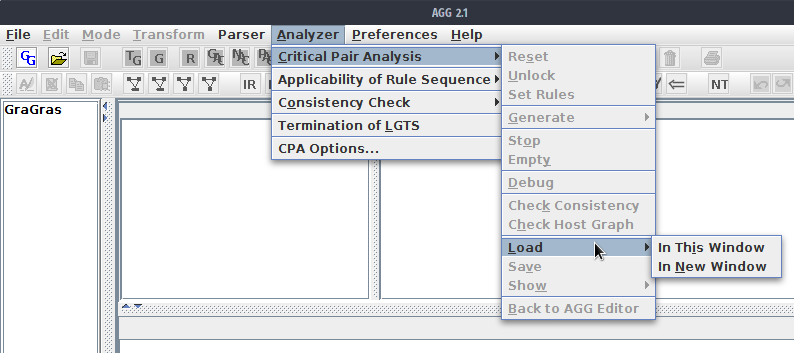
\includegraphics[scale = 0.5]{img/cpa/cpa_01.png}
\end{tutorialstep}

\begin{tutorialstep}
When asked about adding the grammar to the tree view, click yes. Otherwise, AGG will not display the individual conflicts in detail. \\

\noindent
\centering

\includegraphics[scale = 0.6]{img/cpa/cpa_02.png}
\end{tutorialstep}

\begin{tutorialstep}
AGG will display matrices indicating the number of conflicts and dependencies between all pairs of rules. In order to visualize the individual conflicts in detail, click on a cell, for example $(4,4)$ in the conflict matrix. \\

\noindent
\centering
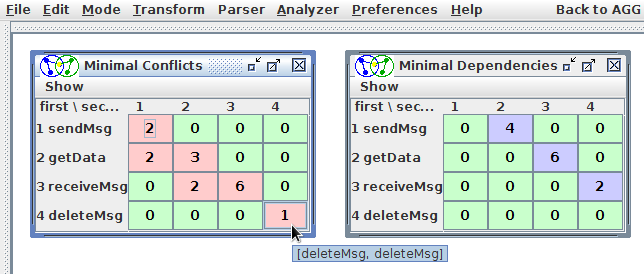
\includegraphics[scale = 0.5]{img/cpa/cpa_03.png}
\end{tutorialstep}

\begin{tutorialstep}
After clicking on the cell, AGG will display the corresponding rules, as well as graphs characterizing the conflicts or dependencies. You may need to rearrange the graphs in order to interpret them. When checking the one conflict between \texttt{deleteMsg} and itself, for example, AGG will show the following graphs, indicating that the conflict occurs when both applications try to delete the same edge between \texttt{data} and \texttt{msg}. \\

\noindent
\centering
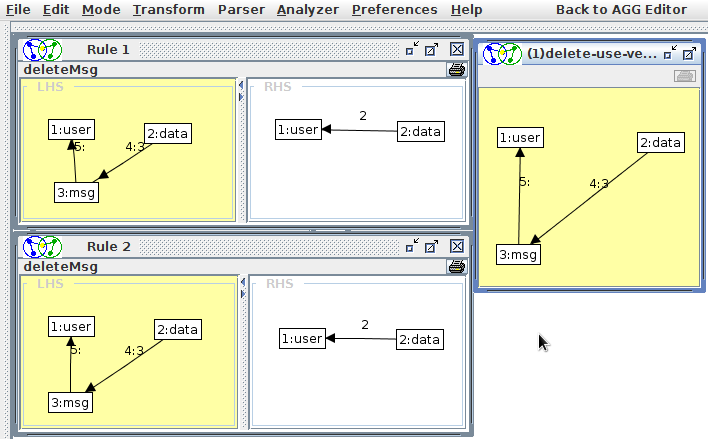
\includegraphics[scale = 0.5]{img/cpa/cpa_04.png}
\end{tutorialstep}

\pagebreak

\section{Concurrent Rules}

\begin{tutorialstep}
  Using \texttt{AGG}, open the file \texttt{grammars/Server/server.ggx}, then right-click on Grammar $>$ New $>$ Rule Sequence. \\

  \noindent
  \centering
  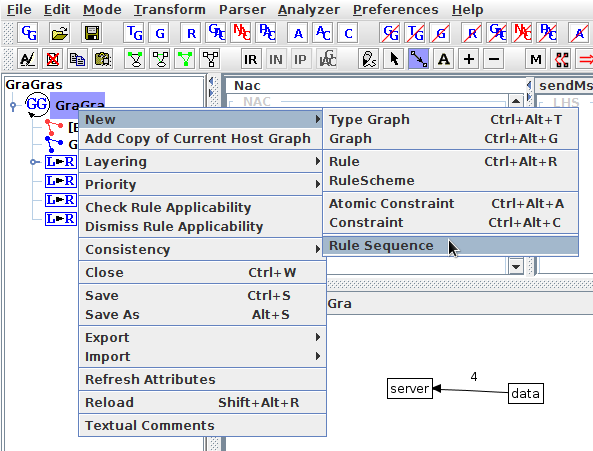
\includegraphics[scale = 0.6]{img/concurrent-rules/rule-sequence_01.png}
\end{tutorialstep}

\begin{tutorialstep}
  Right-click the rule sequence created below the rules of the grammar, then click on \texttt{Show/Edit}, a new pop-up must open.\\

  \begin{center}
  \noindent
  \centering
  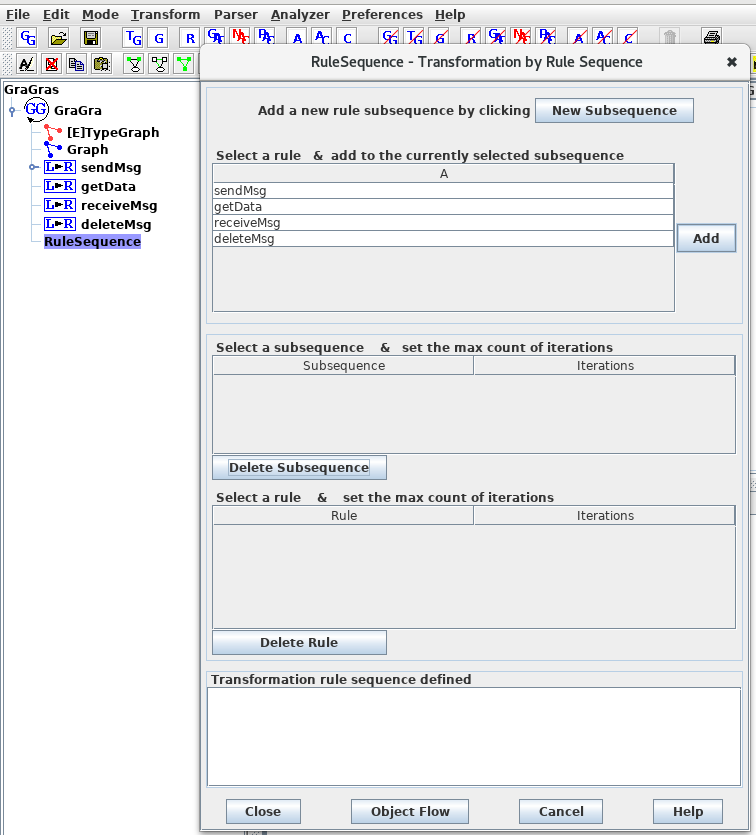
\includegraphics[scale = 0.5]{img/concurrent-rules/rule-sequence_02.png}\\
  \end{center}
  
  Click on \texttt{New Subsequence} button, a new row will be created at the \texttt{Select a subsequence} table. Select the subsequence to add the rules to it.
\end{tutorialstep}

\begin{tutorialstep}

  Once the subsequence was selected, we can add rules to the \texttt{Select a rule} table. Select any rule(s) and click the \texttt{Add} button. You may add a rule multiples times or change its number of \texttt{Iterations} to repeat it. Once the rule sequence is defined, click on close and save the file.\\

  \noindent
  \centering
  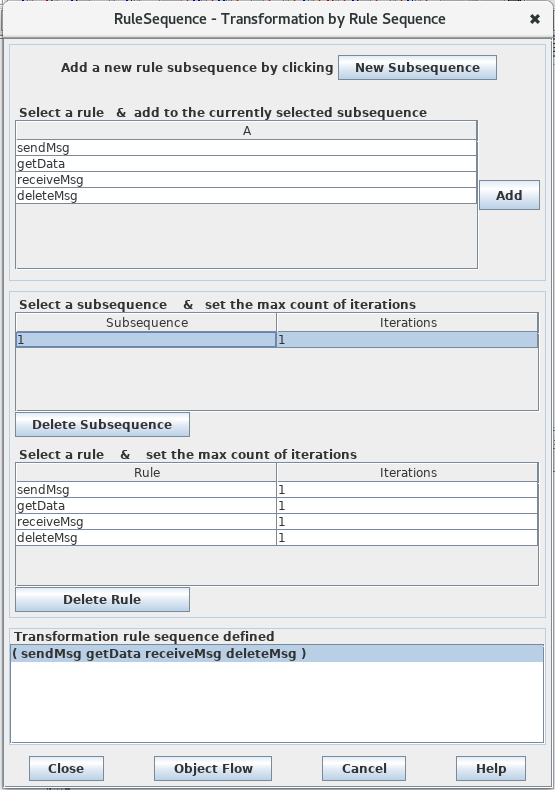
\includegraphics[scale = 0.6]{img/concurrent-rules/rule-sequence_03.png}\\
\end{tutorialstep}

Now, we can use \texttt{verigraph} to compute all the concurrent rules for this rule sequence, using the following command:

\begin{minted}{bash}
$ verigraph concurrent-rule -o output.ggx \
  grammars/Server/server.ggx
\end{minted}

Note that this will generate \emph{all} concurrent rules, which may be a lot (in this particular case 1202 rules), and may take quite some time. We are currently working on using graph constraints and multiplicity to improve the generation of concurrent rules, reducing the number of spurious rules that are generated.

The generated rules are also based on the restriction that matches are always monomorphic. In order to account for arbitrary matches, use the flag \texttt{--all-matches} after the \texttt{verigraph} command.

\subsection{Maximizing Interaction between Rules}

The generated concurrent rules allow for different degrees of interaction between rules, including a parallel rule (where the matched subgraphs are completely disjoint). Sometimes, however, only the concurrent rules with maximum interaction are desired, which may be obtained by the following command:

\begin{minted}{bash}
  $ verigraph concurrent-rule --max-rule -o output.ggx \
    grammars/Server/server.ggx
\end{minted}

\begin{tutorialstep}
  Then open the \texttt{output.ggx} file in \texttt{AGG}, which should have a new rule that looks like this:\\

  \noindent
  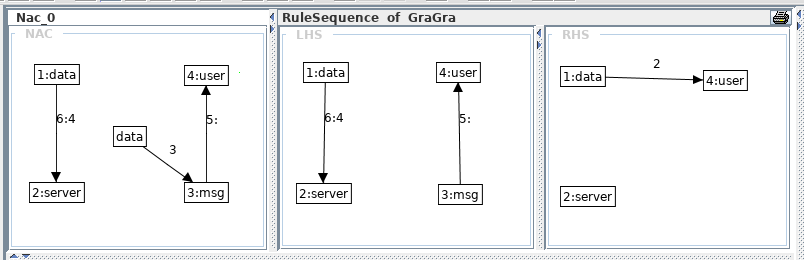
\includegraphics[scale = 0.5]{img/concurrent-rules/rule-sequence_04a.png}\\
  \noindent
  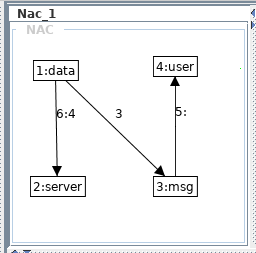
\includegraphics[scale = 0.5]{img/concurrent-rules/rule-sequence_04b.png}\\
\end{tutorialstep}

\subsection{Dependent rules}

Sometimes, maximizing the interaction between rules is an excessively strong restriction. An alternative is generating concurrent rules based on the dependencies between the subsequent rules of a rule sequence. In order to generate such concurrent rules, run:

\begin{minted}{bash}
  $ verigraph concurrent-rule --all-rules --by-dependency -o \ 
  	output.ggx grammars/Server/server.ggx
\end{minted}

The output file must have two new rules, the same one as the previous example, and another that looks like this:\\

\noindent
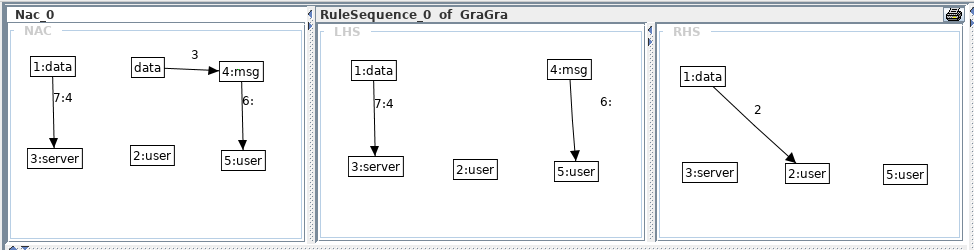
\includegraphics[scale = 0.4]{img/concurrent-rules/rule-sequence_05a.png}\\
\noindent
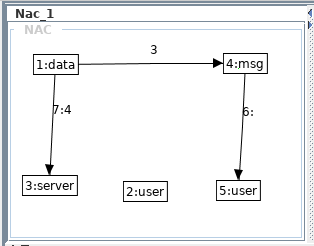
\includegraphics[scale = 0.4]{img/concurrent-rules/rule-sequence_05b.png}\\

\pagebreak

\subsection{Constraints}

It is possible to use positive and negative atomic constraints to restrict the generation of concurrent rules to more significant ones. This is still a \textit{beta} feature that works only with concurrent rules.\\

\begin{tutorialstep}
To add new atomic constraints to a Grammar using \texttt{AGG}, right-click on Grammar $>$ New $>$ Atomic Constraint. \\

  \noindent
  \centering
  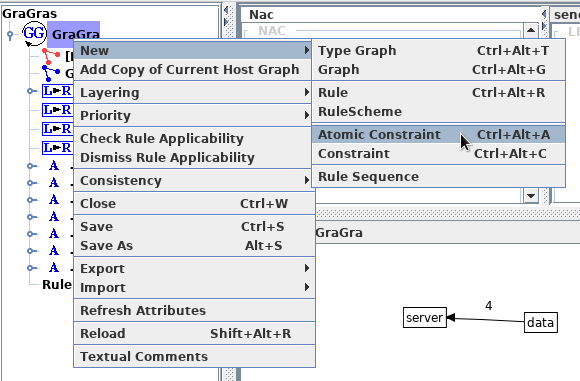
\includegraphics[scale = 0.6]{img/concurrent-rules/atomic_constraints01.png}
\end{tutorialstep}

\begin{tutorialstep}
Click on the newly created atomic constraint to add elements to its \emph{Premise} and \emph{Conclusion} graphs. Notice that  \emph{Verigraph} uses the name of an atomic constraint to interpret it as positive or negative: negative constraints have to start with an $-$ (hyphen), otherwise they are treated as positive. \\

  \noindent
  \centering
  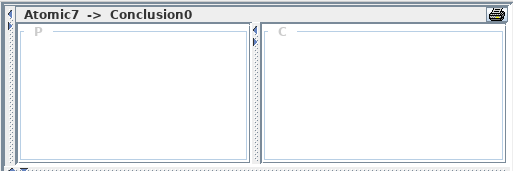
\includegraphics[scale = 0.6]{img/concurrent-rules/new_atomic}
  
\end{tutorialstep}

\pagebreak
\noindent
\textbf{Important:} Although AGG supports adding multiple conclusion graphs to a constraint, Verigraph doesn't.\\

\begin{figure}
  \noindent
  \centering
  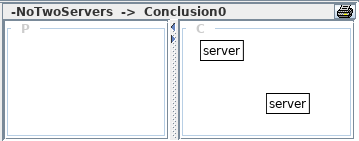
\includegraphics[scale = 0.6]{img/concurrent-rules/new_atomic02}
  \caption{Negative atomic constraint forbidding the existence of more than one server.}
\end{figure}

%% How to use AGG to add atomic constraints

To enable \emph{Verigraph} to use constraints in order to cut off invalid concurrent rules, add the \texttt{--use-constraints} flag before the concurrent rule command. For example:

\begin{minted}{bash}
  $ verigraph --use-constraints concurrent-rule --all-rules \ 
    --by-dependency -o output.ggx grammars/Server/server.ggx
\end{minted}

It can be combined with any previous concurrent rule generation strategy.
%% Gui> sugestão pra deixar bem claro
Note that combining constraints and dependency-induced rules will \emph{not} generate a complete set of rules, since any dependencies caused by the constraints are not not yet calculated by verigraph.

\pagebreak

\section{Second Order}

Although AGG is used for creating the input to \texttt{verigraph}, it does not support second order productions. In order to specify such productions in AGG, we simulate them by using two first order rules, following a naming convention and linking their elements with \emph{Object Names}.\\

{\noindent\centering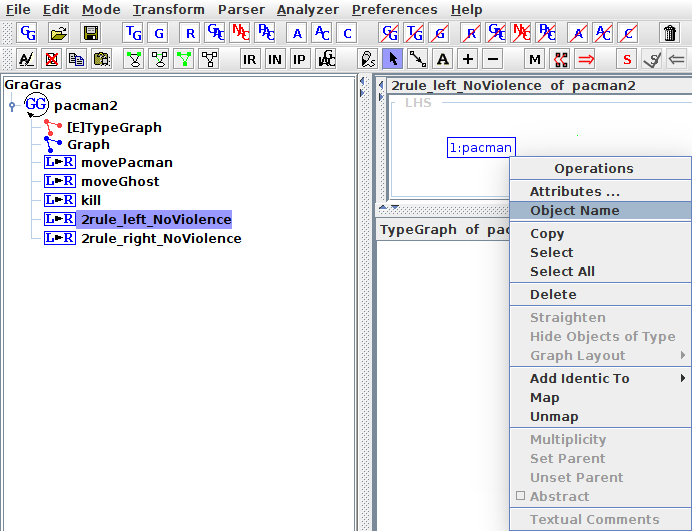
\includegraphics[scale = 0.5]{img/snd-order/objName.png}\\}

The Figure above shows how to set an \emph{Object Name} in a graph element (only numbers are accepted).
The Figure below is a second order production simulated in AGG, the two \emph{pacman} nodes linked have the number 9 in their \emph{Object Name}.

\begin{center}
\noindent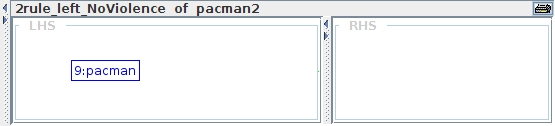
\includegraphics[scale = 0.6]{img/snd-order/noViolenceLeft.png}\\
\noindent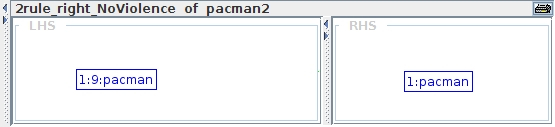
\includegraphics[scale = 0.6]{img/snd-order/noViolenceRight.png}\\
\end{center}

The grammar in \texttt{grammars/Pacman/pacman2.ggx} simulates a simple Pacman game.
This grammar contains the second order production above.
Running the command below will create a new grammar file where all second order productions are applied once on all possible matches of the first order productions.

\begin{minted}{bash}
  $ verigraph snd-order -o output.ggx grammars/Pacman/pacman2.ggx
\end{minted}

The new production below must be on \texttt{output.ggx} file.

{\noindent\centering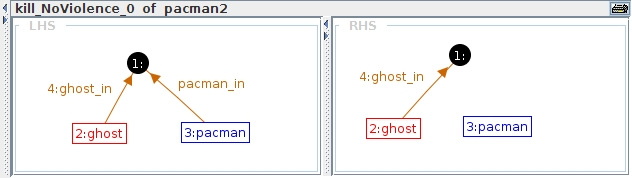
\includegraphics[scale = 0.5]{img/snd-order/kill.png}\\}

\subsection{Inter-level Analysis}

Two new kind analysis arise from inter-level interaction between productions.
These algorithms are being studied, and their implementations are not considered entirely finished, also it lacks of a support GUI.
Despite of it, a log with quantitative information is generated running the command below.

\begin{minted}{bash}
  $ verigraph analysis --snd-order --all-matches \
  	grammars/Pacman/pacman2.ggx
\end{minted}

\pagebreak

\section{Contact Information}

\begin{description}
\item[API internal documentation]:\\ \url{https://verites.github.io/verigraph-docs/}
\item[Reporting issues or suggestions about \emph{Verigraph} and its tutorial]:\\ \url{https://github.com/Verites/verigraph/issues}
\item[Authors' Information]:
\begin{itemize}
\item Andrei Costa: \url{https://inf.ufrgs.br/~acosta/}
\item Guilherme Grochau Azzi: \url{https://inf.ufrgs.br/~ggazzi/}
\item Jonas Santos Bezerra: \url{https://inf.ufrgs.br/~jsbezerra/}
\item Leila Ribeiro: \url{https://inf.ufrgs.br/~leila/}
\item Leonardo Marques Rodrigues
\item Rodrigo Machado: \url{https://inf.ufrgs.br/~rma/}
\end{itemize}

\end{description}



%\begin{minted}{bash}
%  $ verigraph-mcheck
%\end{minted}
\end{document}
